\documentclass[tikz,border=6pt]{standalone}
\usepackage{amsmath,amssymb}
\begin{document}
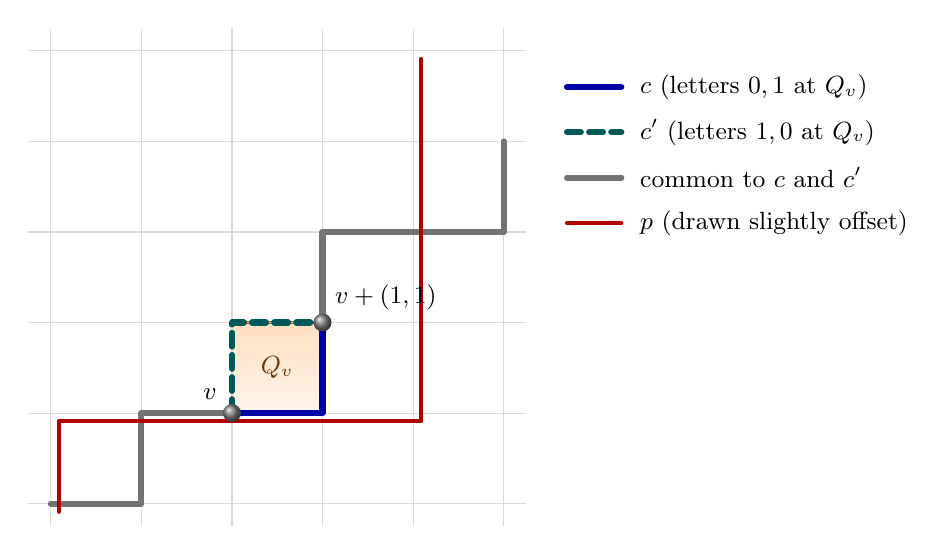
\begin{tikzpicture}[scale=1.15,
  gridl/.style={draw=black!15,line width=0.4pt},
  cpath/.style={draw=blue!65!black,line width=2.2pt,line cap=round,line join=round},
  cpath2/.style={draw=teal!70!black,line width=2.2pt,line cap=round,line join=round,dash pattern=on 5pt off 3pt},
  common/.style={draw=black!55,line width=2.2pt,line cap=round,line join=round},
  ppath/.style={draw=red!70!black,line width=1.5pt,line cap=round,line join=round},
  pt/.style={circle,shading=ball,ball color=#1,inner sep=0pt,minimum size=6.5pt}]
% square Q_v
\shade[top color=orange!25,bottom color=orange!8,draw=orange!70!black,line width=0.9pt] (2,1) rectangle (3,2);
\node[font=\small,orange!40!black] at (2.5,1.5) {$Q_v$};
\foreach \x in {0,...,5} \draw[gridl] (\x,-0.25) -- (\x,5.25);
\foreach \y in {0,...,5} \draw[gridl] (-0.25,\y) -- (5.25,\y);
% common part of c and c'
\draw[common] (0,0) -- (1,0) -- (1,1) -- (2,1);
\draw[common] (3,2) -- (3,3) -- (4,3) -- (5,3) -- (5,4);
% c: E then N around the square; c': N then E
\draw[cpath] (2,1) -- (3,1) -- (3,2);
\draw[cpath2] (2,1) -- (2,2) -- (3,2);
% p: through v, leaves along the bottom side, misses v+(1,1)
\draw[ppath,shift={(0.09,-0.09)}] (0,0) -- (0,1) -- (2,1) -- (3,1) -- (4,1) -- (4,5);
\node[pt=black!50] at (2,1) {};
\node[pt=black!50] at (3,2) {};
\node[font=\small,anchor=south east] at (1.94,1.04) {$v$};
\node[font=\small,anchor=south west] at (3.03,2.03) {$v+(1,1)$};
% legend
\begin{scope}[shift={(5.7,4.6)}]
  \draw[cpath] (0,0) -- (0.6,0); \node[anchor=west,font=\small] at (0.7,0) {$c$ (letters $0,1$ at $Q_v$)};
  \draw[cpath2] (0,-0.5) -- (0.6,-0.5); \node[anchor=west,font=\small] at (0.7,-0.5) {$c'$ (letters $1,0$ at $Q_v$)};
  \draw[common] (0,-1.0) -- (0.6,-1.0); \node[anchor=west,font=\small] at (0.7,-1.0) {common to $c$ and $c'$};
  \draw[ppath] (0,-1.5) -- (0.6,-1.5); \node[anchor=west,font=\small] at (0.7,-1.5) {$p$ (drawn slightly offset)};
\end{scope}
\end{tikzpicture}
\end{document}
